\documentclass[11pt]{article}
\usepackage[scaled=0.92]{helvet}
\usepackage{geometry}
\geometry{letterpaper,tmargin=1in,bmargin=1in,lmargin=1in,rmargin=1in}
\usepackage[parfill]{parskip} % Activate to begin paragraphs with an empty line rather than an indent %\usepackage{graphicx}
\usepackage{amsmath,amssymb, mathrsfs, dsfont}
\usepackage{tabularx}
\usepackage[all,cmtip]{xy}
\usepackage{tikz-cd}
\usepackage[font=footnotesize,labelfont=bf]{caption}
\usepackage{graphicx}
\usepackage{xcolor}
%\usepackage[linkbordercolor ={1 1 1} ]{hyperref}
%\usepackage[sf]{titlesec}
\usepackage{natbib}
%\usepackage{tikz-cd}

\usepackage{../../Tianpei_Report}

%\usepackage{appendix}
%\usepackage{algorithm}
%\usepackage{algorithmic}

%\renewcommand{\algorithmicrequire}{\textbf{Input:}}
%\renewcommand{\algorithmicensure}{\textbf{Output:}}



\begin{document}
\title{Lecture 8: Differentiation}
\author{ Tianpei Xie}
\date{ Aug. 2nd., 2015 }
\maketitle
\tableofcontents
\newpage
\section{Differentiation theorems}
\begin{itemize}
\item \begin{remark}
In these notes we explore the question of the extent to which these theorems continue to hold when the differentiability or integrability
conditions on the various functions $F, F', f$ are relaxed. Among the results proven in these notes are
\begin{enumerate}
\item \emph{\textbf{The Lebesgue differentiation theorem}}, which roughly speaking asserts that \emph{\textbf{the Fundamental Theorem of Calculus}} continues to hold for almost every $x$ if $f$ is merely \emph{\textbf{absolutely integrable}}, rather than \emph{continuous};
\item A number of \emph{differentiation theorems}, which assert for instance that \emph{monotone}, \emph{Lipschitz}, or \emph{bounded variation functions} in one dimension are \emph{\textbf{almost everywhere differentiable}}; and
\item \emph{\textbf{The Second Fundamental Theorem of Calculus}} for \emph{absolutely continuous functions}.
\end{enumerate}
\end{remark}
\end{itemize}
\subsection{The Lebesgue Differentiation Theorem in One Dimension}
\begin{itemize}
\item \begin{theorem} (\textbf{Lebesgue differentiation theorem, one-dimensional case}). \\
Let $f: \bR \rightarrow \bC$ be an \textbf{absolutely integrable} function, and let $F: \bR \rightarrow \bC$ be the definite integral $F(x) := \int_{[-\infty,x]} f(t) dt$. Then $F$ is \textbf{continuous} and \textbf{almost everywhere differentiable}, and $F'(x) = f(x)$ for \textbf{almost every} $x \in \bR$.
\end{theorem}

\item \begin{theorem} (\textbf{Lebesgue differentiation theorem, second formulation}). \\
Let $f: \bR \rightarrow \bC$ be an \textbf{absolutely integrable} function. Then
\begin{align}
 \lim\limits_{h\rightarrow 0+}\frac{1}{h} \int_{[x,x+h]} f(t) dt = f(x) \label{eqn: lebesgue_diff_theo_1}
\end{align} for almost every $x \in \bR$, and
\begin{align}
 \lim\limits_{h\rightarrow 0+}\frac{1}{h} \int_{[x-h,x]} f(t) dt = f(x) \label{eqn: lebesgue_diff_theo_2}
\end{align} for almost every $x \in \bR$.
\end{theorem}

\item \begin{remark} (\emph{\textbf{Density Argument}}) \citep{tao2011introduction} \\
The conclusion \eqref{eqn: lebesgue_diff_theo_1} we want to prove is a \emph{\textbf{convergence theorem}} - an assertion that for all functions $f$ in a given class (in this case, \emph{the class of absolutely integrable functions} $f : \bR \rightarrow \bR$), a certain sequence of \emph{linear expressions} $T_h\,f$ (in this case, \textit{the right averages} $T_h\,f(x) = \frac{1}{h} \int_{[x,x+h]} f(t) dt$) \emph{converge in some sense} (in this case, pointwise almost everywhere) to a specified limit (in this case, $f$).

There is a general and very useful argument to prove such convergence theorems, known as \underline{\emph{\textbf{the density argument}}}. This argument requires
\emph{\textbf{two ingredients}}, which we state informally as follows:
\begin{enumerate}
\item A \emph{\textbf{verification}} of the convergence result for some ``\emph{\textbf{dense subclass}}" of ``\emph{\textbf{nice}}" functions $f$, such as \emph{continuous functions}, \emph{smooth functions}, \emph{simple functions}, etc.. By ``\emph{dense}", we mean that a \emph{general function} $f$ in the \emph{original class} can be \emph{\textbf{approximated to arbitrary accuracy}} in a suitable sense by a function \emph{in the nice subclass}.
\item A \emph{\textbf{quantitative estimate}} that \emph{\textbf{upper bounds}} \emph{the \textbf{maximal fluctuation}} of the \emph{linear expressions} $T_h\,f$ in terms of the ``\emph{\textbf{size}}" of the function $f$ (where \emph{the precise definition of ``size" depends on the nature of the approximation} in the first ingredient).
\end{enumerate} 
Once one has these two ingredients, it is usually not too hard to put them together to obtain the desired convergence theorem for general functions $f$ (\emph{not just those in the dense subclass}). 
\end{remark}

\item \begin{proposition} (\textbf{Translation is continuous} in $L^1$). \citep{tao2011introduction} \\
Let $f : \bR^d \rightarrow \bC$ be an absolutely integrable function, and for each $h \in \bR^d$, let $f_h : \bR^d \rightarrow \bC$ be \textbf{the shifted function} $f_h(x) := f(x - h)$.
Then $f_h$ converges in $L^1$ norm to $f$ as $h \rightarrow 0$, thus
\begin{align*}
\lim\limits_{h \rightarrow 0} \int_{\bR^d} \abs{f_h(x) - f(x)} dx = 0.
\end{align*}
\end{proposition}

\item \begin{exercise}
Let $f, g: \bR^d \rightarrow \bC$ be Lebesgue measurable functions such that $f$ is \textbf{absolutely integrable} and $g$ is \textbf{essentially bounded} (i.e. \textbf{bounded} outside of a null set). Show that \textbf{the convolution} $f * g : \bR^d \rightarrow \bC$ defined by the formula
\begin{align*}
f * g(x) = \int_{\bR^d} f(y)g(x - y) dy
\end{align*} is well-defined (in the sense that the integrand on the right-hand side is absolutely integrable) and that $f * g$ is a \textbf{bounded}, \textbf{continuous} function.
\end{exercise}

\item \begin{remark}
One drawback with \emph{\textbf{the density argument}} is it gives convergence results which are \emph{\textbf{qualitative}} rather than \emph{\textbf{quantitative}} - there is no explicit bound on the rate of convergence.
\end{remark}
\end{itemize}


\subsection{The Lebesgue Differentiation Theorem in $\bR^{d}$}
\subsubsection{Absolute Integrable Version}
\begin{itemize}
\item \begin{theorem}(\textbf{Lebesgue Differentiation Theorem  (Absolute Integrable version)}) \citep{tao2011introduction}\\
Suppose $f: \bR^{d} \rightarrow \bC$ is \textbf{absolutly integrable}. Then for almost every $x$, we have 
\begin{align}
&\lim\limits_{r\rightarrow 0}\frac{1}{m(B(x, r))}\int_{B(x, r)}\abs{f(z) - f(x)}dz = 0 \label{eqn: lebesgue_points}\\
\text{and }\quad & \lim\limits_{r\rightarrow 0}\frac{1}{m(B(x, r))}\int_{B(x, r)}f(z) dz = f(x), \nonumber
\end{align}
where $B(x, r) := \{ y \in \bR^d : \norm{x - y}{} < r\}$ is the open ball of radius $r$ centred at $x$.
\end{theorem}

\item \begin{definition}
A point $x$ for which \eqref{eqn: lebesgue_points} holds is called \emph{\textbf{a Lebesgue point}} of $f$; thus, for an \textbf{\emph{absolutely integrable function}} $f$, \emph{almost every point in $\bR^d$ will be a Lebesgue point for $\bR^d$}.
\end{definition}


\item The \emph{\textbf{quantitative estimate}} we will need is \emph{the Hardy-Littlewood maximal inequality}. First, we need to introduce \emph{the Hardy-Littlewood maximal function}: 
\begin{definition}\citep{folland2013real}\\
If $f\in L_{loc}^{1}(\bR^{d})$, the \underline{\emph{\textbf{Hardy-Littlewood maximal function}}} $Hf(x)$ is defined as
\begin{align*}
Hf(x)&\equiv \sup_{r>0}\frac{1}{m\paren{B(r,x)}}\int_{B(r,x)}\abs{f(z)}dz
\end{align*}
where $B(r,x)= \set{y: \norm{y-x}{}< r}$, and the \emph{\textbf{average value}} of $f$ on $B(r,x)$ is 
\begin{align*}
A_{r}f(x)&=\frac{1}{m\paren{B(r,x)}}\int_{B(r,x)}f(z)dz.
\end{align*}
\end{definition}

\item \begin{remark}
 A useful variant of $Hf(x)$ (see \citep{stein2009real}) as 
\begin{align*}
H^{*}f(x) &\equiv \sup\set{ \frac{1}{m\paren{B}}\int_{B}\abs{f(z)}dz, \;\, B\text{ is a ball }, x\in B  }.
\end{align*}
\end{remark}

\item \begin{remark}
\emph{The Hardy-Littlewood maximal function} is an important function in the field of \emph{(real-variable) harmonic analysis}.
\end{remark}

\item \begin{remark} The Hardy-Littlewood maximal function has the following properties:
\begin{enumerate}
\item $(Hf)^{-1}(a, \infty) = \bigcup_{r>0}(A_{r}f)^{-1}(a,\infty)$ is open for any $a\in \bR$, so the Hardy-Littlewood maximal function is \emph{measureable}. 
\item  Moreover, $Hf(x)<\infty, a.e. x$ is \emph{\textbf{essentially bounded}}.  
\item Note that $Hf \le H^{*}f \le 2^{d}Hf$
\end{enumerate}
\end{remark}

\item We need to prove the following theorem:
\begin{theorem} \label{thm: hardy_littlewood} (\textbf{The Hardy-Littlewood Maximal Theorem}) \citep{stein2009real, folland2013real}\\
Suppose $f$ is integrable, then 
\begin{enumerate}
\item \begin{align*}
H^{*}f(x) &\equiv \sup\set{ \frac{1}{m\paren{B}}\int_{B}\abs{f(z)}dz, \;\, B\text{ is a ball }, x\in B  }.
\end{align*} is measurable. 

\item $H^{*}f(x) <\infty$ for $a.e.\, x$.

\item  $H^{*}f$ satisfies \underline{\textbf{the Hardy-Littlewood maximal inequality}}:
\begin{align*}
m\paren{\set{x: \, H^{*}f(x)> \alpha}} &\le \frac{A}{\alpha}\norm{f}{L^{1}(\bR^{d})}
\end{align*}
for $\alpha>0$, where $A= 3^{d}$, and $\norm{f}{L^{1}(\bR^{d})}= \int_{\bR^{d}}\abs{f(x)}dx$.
\end{enumerate}
Note that $H^{*}f \ge \abs{f}, a.e. x$, but the above expression indicates that \textbf{$H^{*}f$ is not much larger than $\abs{f}$}. However, we may not be able to assume $H^{*}f$ integrable for any $f$.
\end{theorem}

\item \begin{remark}
In order to prove this theorem, we need to introduce concept of \emph{\textbf{Vitali covering}}:
\begin{itemize}
\item \begin{definition}(\emph{\textbf{Vitali Covering}}) \citep{royden1988real, stein2009real}\\
\emph{A collection $\cB$ of balls} $\set{B}$ is said to be a \underline{\emph{\textbf{Vitali covering}}} of a set $E$, (\emph{\textbf{covers $E$ in Vitali sense}},) if for every $x\in E$,  any $\eta>0$, there is a \emph{ball} $B\in \cB$, such that $x\in B$ and $m(B)<\eta$. Thus \emph{every point is covered by \textbf{balls} of \textbf{arbitrary small measure}}.
\end{definition}

\item \begin{lemma}(\textbf{Lebesgue number lemma})\\
For any \textbf{open covering} $\cA$ of the \textbf{metric} space $(X,d)$. If $X$ is \textbf{compact}, there exists a number $\delta>0$ such that for \textbf{any subset} of $X$ having \textbf{diameter} $<\delta$, there exists an element of $\cA$ containing it. 
\end{lemma}

\item \begin{lemma}(\textbf{Vitali Covering Lemma in elementary form}) \citep{stein2009real}\\
Suppose $\cB \equiv \set{B_{1},\ldots, B_{N}}$ is a finite collection of open balls in $\bR^{d}$. Then there exists a disjoint sub-collection $B_{i_{1}}, B_{i_2}, \ldots, B_{i_k}$ of $\cB$ that satisfies
\begin{align*}
m\paren{\bigcup_{s=1}^{N}B_{s}} &\le 3^{d}\sum_{j=1}^{k}m(B_{i_{j}}) 
\end{align*}
Loosely speaking, we may always find \textbf{a disjoint sub-collection of balls} that covers \textbf{a fraction of the region} covered by the original collection of balls. 
\end{lemma}
\begin{proof}
Observe that $B$ and $B'$ is a pair of balls that intersects, with the radius of $B'$ being not greater than that of $B$. Then $B'$ is contained in a ball $\tilde{B}$ that is concentric with $B$ but with $3$ times its radius. 

First, we pick a ball $B_{i_1}$ in $\cB$ with \emph{maximal} (largest) radius, and then delete it from  $\cB$ as well as any ball that intersect with $B_{i_1}$. Thus all deleted balls are contained in the ball $\tilde{B}_{i_1}$ concentric with $B_{i_1}$ with $3$-times its radius.

Then the remaining balls yield a new collection $\cB'$, from which we could repeat the above procedure.  After at most $N$ steps, we obtain a collection of disjoint balls $\tilde{B}_{i_1}, \tilde{B}_{i_2},\ldots, \tilde{B}_{i_k}$.

Finally, we need to prove that the disjoint balls satisfies the above inequality. We use the observation made at the beginning of the proof. Let $\tilde{B}_{i_j}$ be the ball that is concentric to $B_{i_j}$, but with $3$-times its radius. Since any ball $B$ in $\cB$ must a ball $B_{i_j}$ and have equal or smaller radius than $B_{i_j}$, we must have $B\subset \tilde{B}_{i_j}$, thus 
\begin{align*}
m\paren{\bigcup_{s=1}^{N}B_{s}}&\le m\paren{\bigcup_{j=1}^{k} \tilde{B}_{i_j}} \\
&\le \sum_{j=1}^{k}m\paren{\tilde{B}_{i_j}} \\
&= 3^{d}\sum_{j=1}^{k}m\paren{B_{i_j}} 
\end{align*}
In last equality, we use the fact that in $\bR^{d}$ a dilation of a set by $\delta>0$ results in the multiplication of $\delta^{d}$ of the Lebesgue measure. \qed
\end{proof}


\item We will use the following \emph{Vitali Covering Lemma} to prove \emph{the Hardy-Littlewood maximal theorem}: 
\begin{lemma} (\textbf{Vitali Covering Lemma in general})  \citep{stein2009real, folland2013real}\\
Suppose $E$ is a set of finite measure and $\cB$ is a Vitali covering of $E$. For any $\delta>0$, we can find finitely many balls $B_{1},\ldots, B_{N}$ in $\cB$ that are disjoint and so that 
\begin{align*}
\sum_{i=1}^{N}m(B_{i}) &\ge m(E) - \delta
\end{align*}
\end{lemma}
\begin{proof}
We can apply the elementary lemman above iteratively, with the aim of exhausting the set $E$. It suffice to take $\delta$ sufficiently small, say $\delta < m(E)$, and using the just cited covering lemma, we can find an initial collection of disjoint balls $B_{1}, \ldots, B_{N_1}$ in $\cB$ such that $\sum_{i=1}^{N_1}m(B_{i}) \ge \gamma\delta$, where $\gamma = 3^{-d}$.

Indeed, first we have $m(E')\ge \delta$ for an appropriate compact subset $E'$ of $E$. Because of the compactness, we can cover $E'$ with finitely many balls from $\cB$, and then the previous lemma allows us to select a disjoint sub-collection of these balls $B_{1}, B_{2}, \ldots, B_{N_1}$ such that $\sum_{i=1}^{N_1}m(B_{i}) \ge \gamma\,m(E')\ge \gamma\delta$. 

With $B_{1}, \ldots, B_{N_1}$ as our initial sequence of balls, we consider two possibilities: either $\sum_{i=1}^{N_1}m(B_{i}) $ $\ge m(E)- \delta$ and we are done with $N= N_1$; or, contrariwise,  $\sum_{i=1}^{N_1}m(B_{i}) < m(E)- \delta$. In the second case, with $E_{2} = E - \bigcup_{i=1}^{N_1}\overline{B}_{i}$ so that $m(E_2)> \delta$. We then repeat the above procedure, by choosing a compact subset $E^{'}_{2}$ of $E_{2}$ with $m(E^{'}_{2})> \delta$, and by noting that the balls in $\cB$ that are disjoint from $\bigcup_{i=1}^{N_1}\overline{B}_{i}$ still cover $E_{2}$ and in fact gives a Vitali covering of $E_{2}$, and hence for $E'_{2}$. Then we can choose $B_{i}, N_{1}< i\le N_{2}$ so that $\sum_{i=N_{1}}^{N_2}m(B_{i}) \ge \gamma\delta$. Therefore, now $\sum_{i=1}^{N_2}m(B_{i}) \ge 2\gamma\delta$ and balls $B_{i}, 1\le i\le N_{2}$ are disjoint. 

Again we consider whether or not $\sum_{i=1}^{N_2}m(B_{i})\ge m(E)- \delta$: if it is $N=N_2$; otherwise repeat for $E_{3}= E-  \bigcup_{i=1}^{N_2}\overline{B}_{i}$. If $k\ge (m(E)-\delta)/(\gamma\delta)$, then after at most $k$-steps, we should have selected a subcollection of disjoint balls $B_{i}, 1\le i\le N_{k}$ with its sum of measures  $\ge k\gamma\delta$. Thus \begin{align*}
\sum_{i=1}^{N_{k}}m(B_{i}) &\ge m(E) - \delta,
\end{align*} which completes our proof. \qed
\end{proof}

\item \begin{corollary} \citep{stein2009real, royden1988real}\\
Follwing the setting above, we can arrange the choice of balls so that
\begin{align*}
m\paren{E- \bigcup_{i=1}^{N}B_{i}} &< 2\delta
\end{align*}
\end{corollary}
\begin{proof}
Let $O\supset E$ be an open set that contains $E$ with $m(O-E)<\delta$. We then choose balls that are contained in $O$. Then $(E- \bigcup_{i=1}^{N}B_{i})\cup \bigcup_{i=1}^{N}B_{i} \subset O$. 
\begin{align*}
m\paren{E- \bigcup_{i=1}^{N}B_{i}} &\le m(O)- m\paren{\bigcup_{i=1}^{N}B_{i}}\\
&\le m(E) + \delta - (m(E)-\delta) = 2\delta.\qed
\end{align*}
\end{proof}
\end{itemize}
\end{remark}

\item Now we turn to the proof of Theorem \ref{thm: hardy_littlewood}
\begin{proof}
\begin{enumerate}
\item Note that the set $E_{\alpha} = \set{x: H^{*}f(x)> \alpha}$ is open, because if $\overline{x}\in E_{\alpha} $, then there exists a ball $B$ such that $\overline{x}\in B$ and
\begin{align*}
\frac{1}{m\paren{B}}\int_{B}\abs{f(z)}dz >\alpha.
\end{align*}
Now any $x$ close enough to $\overline{x}$ will also belong to $B$; hence $x\in E_{\alpha}$ as well. 

\item Follows from the fact that $\set{x: H^{*}f(x)= \infty}= \bigcap_{\alpha=1}^{\infty}\set{x: H^{*}f(x)> \alpha}$. So the measure approaches to $0$ as $\alpha\rightarrow \infty$. 

\item Use \emph{\textbf{the Vitali covering lemma}}. Let $E_{\alpha}=\set{x: H^{*}f(x)> \alpha} $. For each $x\in E_{\alpha}$, there exists a ball $B_{x}$ that contains $x$, and 
\begin{align*}
\frac{1}{m\paren{B_{x}}}\int_{B_{x}}\abs{f(z)}dz&>\alpha.
\end{align*}
So for each ball 
\begin{align*}
m\paren{B_{x}} &< \frac{1}{\alpha}\int_{B_{x}}\abs{f(z)}dz.
\end{align*}
Fix a compact subset $K$ of $E_{\alpha}$. Since $K$ is covered by $\bigcup_{x\in E_{\alpha}}B_{x}$, we have a finite subcover $K\subset \bigcup_{m=1}^{N}B_{m}$. The covering lemma guarantees the existence of a subcollection $B_{i_1}, \ldots, B_{i_k}$ of disjoint balls with 
\begin{align*}
m\paren{\bigcup_{m=1}^{N}B_{m}} &\le 3^{d} \sum_{j=1}^{k}m(B_{i_j}). 
\end{align*}
Then
\begin{align*}
m(K) \le m\paren{\bigcup_{m=1}^{N}B_{m}} &\le 3^{d} \sum_{j=1}^{k}m(B_{i_j})\\
&\le \frac{3^{d}}{\alpha}\sum_{j=1}^{k}\int_{B_{i_j}}\abs{f(z)}dz\\
&= \frac{3^{d}}{\alpha}\int_{\bigcup_{j=1}^{k}B_{i_j}}\abs{f(z)}dz \quad (B_{i_j} \text{ are disjoint})\\
&\le  \frac{3^{d}}{\alpha}\int_{\bR^{d}}\abs{f(z)}dz
\end{align*}

Since the above inequality holds for all $K\subset E_{\alpha}$ compact, we use the inner regularity of Lebesgue measure, 
\begin{align*}
m(E_{\alpha}) =\sup_{K\subset E_{\alpha}, \text{ compact}}m(K) &\le  \frac{3^{d}}{\alpha}\int_{\bR^{d}}\abs{f(z)}dz.\qed
\end{align*}
\end{enumerate}
\end{proof}
\end{itemize}

\subsubsection{Local Integrable Version}
\begin{itemize}
\item \begin{definition}\citep{stein2009real}\\
A \emph{measurable function} $f$ on $\bR^{d}$ is \emph{\textbf{locally integrable}}, i.e. $f\in L_{loc}^{1}(\bR^{d})$, if for every ball $B$ the function $f(x)\mathds{1}_{B}$ is \emph{integrable}. 
\end{definition}

\item This theorem follows from \emph{the Hardy-Littlewood maximal inequality}
\begin{theorem}  \citep{stein2009real}\\
If $f\in L_{loc}^{1}(\bR^{d})$ is \textbf{locally integrable}, then for the \textbf{average} of $f$, i.e. 
\begin{align*}
A_{r}f(x)&=\frac{1}{m\paren{B(r,x)}}\int_{B(r,x)}f(z)dz,\\
\end{align*} we have
\begin{align*}
A_{r}f(x) \stackrel{a.e.}{\rightarrow} f(x), \quad r\rightarrow 0. 
\end{align*}
\end{theorem}
\begin{proof}
It suffices to show that for $N\in \bN$, $A_{r}f(x)  \rightarrow f(x)$ for $a.e. x$ with $\abs{x}\le N$. But for $\abs{x}\le N$ and $r\le 1$ the values $A_{r}f(x)$ depend only on values $f(z)$ for $\abs{z} \le N+1$, so by replacing $f$ with $f\ind{B(N+1, 0)}$ we may assume that that $f\in L^{1}$.

Given $\epsilon >0$, we know that there exists a continuous integrable function $g$ such that $\int \abs{g(z)- f(z)}dz$ $<\epsilon $. Continuity of $g$ implies that for every $x\in \bR^{d}$ and $\delta >0$, there exists $r>0$ such that $\abs{g(y)- g(z)}<\delta$ whenever $\abs{y-x}<r$, and hence, 
\begin{align*}
\abs{A_{r}g(x) - g(x) }&= \frac{1}{m\paren{B(r,x)}}\abs{\int_{B(r,x)}\brac{g(z)- g(x)}dz}<\delta. 
\end{align*}
Therefore $A_{r}g(x) \rightarrow g(x)$ as $r\rightarrow 0$ for every $x$, so
\begin{align*}
\limsup\limits_{r\rightarrow 0}\abs{A_{r}f(x) - f(x)}
&= \limsup\limits_{r\rightarrow 0}\abs{A_{r}(f-g)(x)+  A_{r}g(x) - g(x) + g(x)- f(x)}\\
&\le H(f-g)(x)+ 0+ \abs{f-g}(x).
\end{align*}
Hence, if
\begin{align*}
F_{\alpha} &= \set{x: \limsup\limits_{r\rightarrow 0}\abs{A_{r}f(x) - f(x)}>\alpha}, \\
G_{\alpha} &=  \set{x: \abs{f-g}(x)>\alpha},
\end{align*}
we have 
\begin{align*}
F_{\alpha} \subset G_{\alpha/2} \cup \set{x: H(f-g)>\alpha/2}.
\end{align*}
But $\frac{\alpha}{2} m(G_{\alpha/2} ) \le \int_{G_{\alpha/2}}\abs{f(x)- g(x)}dx < \epsilon$, so by the maximal theorem, 
\begin{align*}
m(F_{\alpha}) &\le \frac{2\epsilon}{\alpha}+ \frac{2A\epsilon}{\alpha}.
\end{align*}
Since $\epsilon>0$ is arbitrary, $m(F_{\alpha})=0$ for all $\alpha>0$. But $\lim\limits_{r\rightarrow 0}A_{r}f(x)= f(x)$ for all $x\in \bigcup_{n=1}^{\infty}E_{1/n}$, so we have done. \qed
\end{proof}

\item \begin{definition}\citep{stein2009real}\\
If $f\in L_{loc}^{1}(\bR^{d})$, the \emph{\textbf{Lebesgue set}} of $f$ consists of all points $\overline{x}\in \bR^{d}$ for which $f(\overline{x})$ is \emph{\textbf{finite}} and 
\begin{align*}
\lim\limits_{m(B)\rightarrow 0\atop \overline{x}\in B}\frac{1}{m\paren{B}}\int_{B}\abs{f(z)- f(\overline{x})}dz &= 0.
\end{align*}
or \emph{equivalently}, \citep{folland2013real},
\begin{align*}
Lf &\equiv\set{x\in \bR^{d}: \lim\limits_{r\rightarrow 0}\frac{1}{m\paren{B(r,x)}}\int_{B(r,x)}\abs{f(z)- f(x)}dz = 0}.
\end{align*}
\end{definition}

\item \begin{corollary}
Suppose $E$ is a measureable set in $\bR^{d}$. Then
\begin{enumerate}
\item Almost every $x\in E$ is \textbf{a point of Lebesgue density} of $E$;
\item Almost every $x\not\in E$ is \textbf{not a point of Lebesgue density} of $E$.
\end{enumerate}
\end{corollary}

\item \begin{corollary}
If $f$ is \textbf{locally integrable} on $\bR^{d}$, then \textbf{almost every point} belongs to\textbf{ the Lebesgue set} of $f$. 
\end{corollary}
\begin{proof}
Apply the theorem above to $\abs{f(z)- q}$ shows that for each rational $q$, there exists a set $E_{q}$ of measure $0$ such that 
\begin{align*}
\lim\limits_{r\rightarrow 0}\frac{1}{m\paren{B(r,x)}}\int_{B(r,x)}\abs{f(z)-q}dz &= \abs{f(x)-q}
\end{align*} for all $x\not\in E_{q}$.

If $E= \bigcup_{q\in \bQ}E_{q}$, then $m(E) = 0$. Now suppose that $x\not\in E$.  Given $\epsilon >0$, there exists a rational $q$ such that $\abs{f(x)- q}<\epsilon $. Since 
\begin{align*}
\frac{1}{m\paren{B(r,x)}}\int_{B(r,x)}\abs{f(z)- f(x)}dz&\le \frac{1}{m\paren{B(r,x)}}\int_{B(r,x)}\abs{f(z)-q}dz +   \abs{f(x)-q}, 
\end{align*}
we must have
\begin{align*}
\limsup\limits_{r\rightarrow 0}\frac{1}{m\paren{B(r,x)}}\int_{B(r,x)}\abs{f(z)- f(x)}dz&\le 2\epsilon, 
\end{align*}
and thus $x$ is in the Lebesgue set of $f$. \qed 
\end{proof}

\item \begin{definition}
A collection of sets $\set{U_{\alpha}}$ is said to \emph{\textbf{shrink regularly}} to $\overline{x}$ or has \emph{\textbf{bounded eccentricity}} at $\overline{x}$ if there is a constant $c>0$ such that for each $U_{\alpha}$ there is a ball $B$ with 
\begin{align*}
\overline{x}\in B, \qquad U_{\alpha} \subset B,  \qquad m(U_{\alpha}) \ge c\,m(B). 
\end{align*}
\end{definition}

\item \begin{theorem}(\textbf{Lebesgue Differentiation Theorem (Local Integrable version)}) \citep{stein2009real, folland2013real}\\
Suppose $f$ is \textbf{locally integrable} on $\bR^{d}$. For every $x$ in the Lebesgue set of $f$, i.e. for almost every $x$, we have 
\begin{align*}
&\lim\limits_{m(U_{\alpha})\rightarrow 0\atop x\in U_{\alpha}}\frac{1}{m(U_{\alpha})}\int_{U_{\alpha}}\abs{f(z) - f(x)}dz = 0\\
\text{and }&\lim\limits_{m(U_{\alpha})\rightarrow 0\atop x\in U_{\alpha}}\frac{1}{m(U_{\alpha})}\int_{U_{\alpha}}f(z) dz = f(x),
\end{align*}
for every family $\set{U_{\alpha}}$ that \textbf{shrinks regularly} to $x$.
\end{theorem}
\begin{proof}
See that if $x\in B$ with $U_{\alpha} \subset B$ and $m(U_{\alpha})\ge c m(B)$, then 
\begin{align*}
\frac{1}{m(U_{\alpha})}\int_{U_{\alpha}}\abs{f(z) - f(x)}dz&\le \frac{1}{c \,m(B)}\int_{B}\abs{f(z) - f(x)}dz<\epsilon
\end{align*} which follows from the fact that $x$ is in the Lebesgue set of $f$.\qed
\end{proof}
\end{itemize}

\subsection{Lebesgue Density and Radon-Nikodym Derivative}
\begin{itemize}
\item Now we turn to consequences of \emph{the Lebesgue differentiation theorem}. 
\begin{definition}\citep{stein2009real}\\
If $E$ is a measureable set in $\bR^{d}$, $x\in \bR^{d}$ is a \underline{\emph{\textbf{point of Lebesgue density}}} of $E$ if
\begin{align*}
\lim\limits_{m(B)\rightarrow 0 \atop x\in B}\frac{m(B\cap E)}{m(B)} &= 1.
\end{align*} 
\emph{Loosely speaking}, it says that a small ball contains $x$ are \emph{almost entirely covered by $E$}. Then for any $\alpha<1$ close to $1$, and \emph{every ball of \textbf{sufficiently small radius}} containing $x$, we have
\begin{align*}
m(E\cap B) &\ge \alpha\, m(B).
\end{align*}
\end{definition}

\item \begin{definition} 
A Borel \emph{measure} $\nu$ on $\bR^d$ will be called \emph{\textbf{regular}} if
\begin{enumerate}
\item $\nu(K) < \infty$ for every \emph{\textbf{compact}} $K$;
\item $\nu(E) = \inf\{\nu(U): U\text{ open}, E \subseteq U\}$ for every $E \in \cB[\bR^{d}]$.
\end{enumerate}
(Condition (2) is actually implied by condition (1). \emph{A \textbf{signed} or \textbf{complex} Borel measure $\nu$} will be called \emph{\textbf{regular}} if $\abs{\nu}$ is \emph{regular}.
\end{definition}

\item \begin{theorem}(\textbf{Lebesgue Density from Radon-Nikodym derivative}) \citep{folland2013real}\\
Let $\nu$ be a \textbf{regular signed measure} on $\bR^{d}$, and let $d\nu = d\lambda+ fdm$ be its Lebesgue-Radon-Nikodym decomposition, where $\lambda \perp m$.  Then for $m$-almost every $x\in \bR^{d}$,
\begin{align*}
\lim\limits_{r\rightarrow 0}\frac{\nu(E_{r})}{m(E_{r})} &= f(x),
\end{align*} where $E_{r}$ \textbf{shrinks regularly} to $x$.
\end{theorem}
\begin{proof}
It is easy to verify that $d\abs{v}= d\abs{\lambda}+ fdm$, so the regularity of $\nu$ implies the regularity of $\lambda$ and $fdm$. In particular, $f\in L_{loc}^{1}$. From differentiation theorem, for $m$-almost every $x\in \bR^{d}$,
\begin{align*}
\lim\limits_{r\rightarrow 0}\frac{\int \ind{E_{r}}fdm}{m(E_{r})} &= f(x).
\end{align*}
Then it suffice to show that for $\lambda \perp m$, $\lambda$ regular, 
\begin{align*}
\lim\limits_{r\rightarrow 0}\frac{\lambda(E_{r})}{m(E_{r})} &= 0.
\end{align*}
Note that $E_{r} \subset B(r,x)$ with $m(E_{r})\ge c B(r,x)$, so 
\begin{align*}
\frac{\lambda(E_{r})}{m(E_{r})} \le \frac{\abs{\lambda}(E_{r})}{m(E_{r})}&\le   \frac{\abs{\lambda}(B(r,x))}{m(E_{r})}
\le  \frac{\abs{\lambda}(B(r,x))}{c m(B(r, x))}.
\end{align*}
Therefore, it suffice to assume that $\lambda$ is positive measure, with $E_{r}$ replaced by $B(r,x)$. Let $A$ be the Borel set that $\lambda(A)= m(A^{c})= 0$, and 
\begin{align*}
F_{k}&\equiv  \set{x\in A:  \limsup\limits_{r\rightarrow 0}\frac{\lambda(B(r,x))}{m(B(r,x))} \ge \frac{1}{k} }.
\end{align*} It suffice to show that $m(F_{k})= 0$ for all $k$.

By regularity of $\lambda$, there is an open $U_{\epsilon} \supset A$ such that $\lambda(U_{\epsilon})<\epsilon$. Each $x\in F_{k}$ is the center of a ball $B_{x} \subset U_{\epsilon}$  such that $\lambda(B_{x}) > \frac{1}{k}m(B_{x})$. Let $V_{\epsilon} = \bigcup_{x\in F_{k}}B_{x}$ and $c< m(V_{\epsilon})$, there exists $x_{1}, \ldots, x_{J}$ such that $B_{x_1},\ldots, B_{x_J}$ are disjoint and 
\begin{align*}
c < m(V_{\epsilon})\le 3^{d}\sum_{k=1}^{J}m(B_{x_{k}}) &\le 3^{d}k\sum_{k=1}^{J}\lambda(B_{x_{k}})\le  3^{d}k\lambda(V_{\epsilon})
\le 3^{d}k\lambda(U_{\epsilon}) \le 3^{d}k\epsilon. 
\end{align*}
So $m(V_{\epsilon})\le 3^{d}k\epsilon$, and since $F_{k}\subset V_{\epsilon}$, $\epsilon$ is arbitrary, then $m(F_{k})= 0$.\qed
\end{proof}
\end{itemize}

\section{The Fundamental Theorem of Calculus for Lebesgue Integral}
\subsection{Functions of Bounded Variations}
\begin{itemize}
\item \begin{theorem} (\textbf{Monotone Differentiation Theorem}). \citep{tao2011introduction} \\
Any function $F : \bR \rightarrow \bR$ which is \textbf{monotone} (either monotone non-decreasing or monotone non-increasing) is \textbf{differentiable almost everywhere}.
\end{theorem}

\item \begin{definition} (\textbf{\emph{Jump function}}). \citep{tao2011introduction}\\
\emph{A \textbf{basic jump function}} $J$ is a function of the form
\begin{align*}
J(x) &:= \left\{
\begin{array}{cc}
0 &\text{when }x < x_0 \\
\theta &\text{when }x = x_0 \\
1 &\text{when }x > x_0
\end{array}
\right.
\end{align*}
for some real numbers $x_0 \in \bR$ and $0 \le \theta \le 1$; we call $x_0$ \emph{\textbf{the point of discontinuity}} for $J$ and $\theta$ \emph{\textbf{the fraction}}. Observe that such functions are \emph{\textbf{monotone non-decreasing}}, but have a \emph{\textbf{discontinuity}} at one point.

\emph{A \textbf{jump function}} is any \emph{\textbf{absolutely convergent} combination of basic jump functions}, i.e. a function of the form $F = \sum_{n}c_n\,J_n$, where $n$ ranges over an \emph{at most countable set}, each $J_n$ is \emph{a basic jump function}, and the $c_n$ are \emph{\textbf{positive} reals} with $\sum_n c_n < \infty$. If there are \emph{only \textbf{finitely many}} $n$ involved, we say that $F$ is a \emph{\textbf{piecewise constant jump function}}.
\end{definition}

\begin{example}
If $q_1, q_2, q_3, \ldots$ is any enumeration of the \emph{rationals}, then $\sum_{n=1}^{\infty} 2^{-n}\mathds{1}_{[q_n,+\infty)}$ is \emph{a jump function}.
\end{example}


\item \begin{remark}
\emph{\textbf{All jump functions are monotone non-decreasing}}.  

From the absolute convergence of the $c_n$ we see that \emph{\textbf{every jump function is the uniform limit of piecewise constant jump functions}}, for instance
$\sum_{n=1}^{\infty}c_n\,J_n$ is the uniform limit of $\sum_{n=1}^{N}c_n\,J_n$. One consequence of this is that the \emph{points of discontinuity of a jump function} $\sum_{n=1}^{\infty}c_n\,J_n$ are \emph{precisely those of the individual summands} $c_n\,J_n$, i.e. \emph{of the points $x_n$ where each $J_n$ jumps}.
\end{remark}

\item The key fact is that \emph{these \textbf{Jump functions}}, together with \emph{\textbf{the continuous monotone functions}}, \emph{\textbf{essentially generate all monotone functions}}, at least \emph{in the bounded case}:
\begin{lemma} (\textbf{Continuous-singular decomposition for monotone functions}). \\
Let $F : \bR \rightarrow \bR$ be a \textbf{monotone non-decreasing} function.
\begin{enumerate}
\item The only \textbf{discontinuities} of F are \textbf{jump discontinuities}. More precisely, if $x$ is a point where $F$ is discontinuous, then the
limits $\lim_{y\rightarrow x^{-}}F (y)$ and $\lim_{y\rightarrow x^{+}}F (y)$ both exist, but are \textbf{unequal}, with $\lim_{y\rightarrow x^{-}}F (y) < \lim_{y\rightarrow x^{+}}F (y)$.
\item There are at most \textbf{countably} many \textbf{discontinuities} of $F$.
\item If $F$ is \textbf{bounded}, then $F$ can be expressed as the \textbf{sum} of a \textbf{continuous} \textbf{monotone non-decreasing function} $F_c$ and a \textbf{jump function} $F_{pp}$.
\end{enumerate}
\end{lemma}

\item \begin{exercise}
Show that the decomposition of a bounded monotone non-decreasing function $F$ into continuous $F_c$ and jump components $F_{pp}$ given by the above lemma is unique.
\end{exercise}



\item \begin{remark}
Just as the \emph{integration theory} of \emph{unsigned functions} can be used to develop \emph{the integration theory} of the \emph{absolutely convergent functions}, the \emph{\textbf{differentiation theory}} of \emph{\textbf{monotone functions}} can be used to develop a parallel \emph{differentiation theory} for the class of \emph{\textbf{functions of bounded variation}}:
\end{remark}

\item \begin{definition} (\emph{\textbf{Bounded variation}}).\\
Let $F : \bR \rightarrow \bR$  be a function. \underline{\emph{\textbf{The total variation}}} $\norm{F}{TV(\bR)}$ (or $\norm{F}{TV}$ for short) of $F$ is
defined to be the \emph{\textbf{supremum}}
\begin{align*}
\norm{F}{TV(\bR)} := \sup\limits_{x_0 \xdotx{<} x_n}\sum_{i=1}^{n}\abs{F(x_i) - F (x_{i-1})}
\end{align*} where the supremum ranges over all \textbf{\emph{finite increasing sequences}} $x_0 \xdotx{,} x_n$ of real numbers with $n \ge 0$; this is a quantity in $[0, +\infty]$. We say that \underline{\emph{\textbf{$F$ has bounded variation (on $\bR$)}}} if $\norm{F}{TV(\bR)}$ is \emph{\textbf{finite}}. (In this case, $\norm{F}{TV(\bR)}$ is often written as $\norm{F}{BV(\bR)}$ or just $\norm{F}{BV}$.)
\end{definition}

\item \begin{remark}
Given any \emph{\textbf{interval}} $[a, b]$, we define \emph{\textbf{the total variation}} $\norm{F}{TV([a, b])}$ of $F$ on $[a, b]$ as
\begin{align*}
\norm{F}{TV(\bR)} := \sup\limits_{a\le x_0 \xdotx{<} x_n \le b}\sum_{i=1}^{n}\abs{F(x_i) - F (x_{i-1})}
\end{align*} We say that a function $F$ has \emph{\textbf{bounded variation on $[a, b]$}} if $\norm{F}{BV([a,b])}$ is \emph{finite}. Note that $\norm{F}{TV(\bR)} = \lim_{N\rightarrow \infty}\norm{F}{TV([-N, N])}$.
\end{remark}

\item \begin{proposition}
If $F : \bR \rightarrow \bR$ is a \textbf{monotone function},  $\norm{F}{TV([a, b])}= \abs{F(b) - F(a)}$ for any interval $[a, b]$. Thus $F$ has
\textbf{bounded variation} on $\bR$ if and only if it is \textbf{bounded}.
\end{proposition}

\item \begin{proposition}
For any functions $F, G: \bR \rightarrow \bR$, the total variation $\norm{\cdot}{TV(\bR)}$ satisfies the following property:
\begin{enumerate}
\item (\textbf{Non-Negativity}): $\norm{F}{TV(\bR)} \ge 0$; 
\item (\textbf{Positive Definiteness}): $\norm{F}{TV(\bR)} = 0$ if and only if $F$ is constant.
\item (\textbf{Homogeneity}): $\norm{c\,F}{TV(\bR)} =\abs{c}\,\norm{F}{TV(\bR)}$ for any $c \in \bR$.
\item (\textbf{Triangle Inequality}): $\norm{F + G}{TV(\bR)} \le \norm{F}{TV(\bR)} + \norm{G}{TV(\bR)}$
\end{enumerate} Thus $\norm{\cdot}{TV(\bR)}$ is a \textbf{norm}.
\end{proposition}

\item \begin{exercise} (Bounded Variation is \textbf{Stronger} than Bounded)
\begin{enumerate}
\item Show that every function $f : \bR \rightarrow \bR$ of \textbf{bounded variation} is \textbf{bounded}, and that the limits $\lim_{x\rightarrow+\infty} f(x)$
and $\lim_{x\rightarrow-\infty} f(x)$, are well-defined.
\item Give a counterexample of a \textbf{bounded}, \textbf{continuous}, \textbf{compactly supported} function $f$ that is \textbf{not} of \textbf{bounded variation}.
\end{enumerate}
\end{exercise}

\item 
\begin{proposition}
A function $F : \bR \rightarrow \bR$ is of \textbf{bounded variation} if and only if it is the \textbf{difference} of two \textbf{bounded monotone functions}.
\end{proposition}

\item \begin{remark}
Much as \emph{an absolutely integrable function} can be expressed as the difference of its \emph{positive} and \emph{negative parts}, \emph{\textbf{a bounded variation function}} can be expressed as \emph{\textbf{the difference of two bounded monotone functions}}. Let
\begin{align*}
F^{+}(x) &=  \sup\limits_{x_0 \xdotx{<} x_n \le x}\sum_{i=1}^{n}\max\{F(x_i) - F (x_{i-1}), 0\}\\
F^{-}(x) &=  \sup\limits_{x_0 \xdotx{<} x_n \le x}\sum_{i=1}^{n}\max\{-F(x_i) + F (x_{i-1}), 0\}
\end{align*}
We have 
\begin{align*}
F(x) &= F(-\infty) + F^{+}(x) - F^{-}(x)\\
\norm{F}{TV([a, b])}  &= F^{+}(b) - F^{+}(a) + F^{-}(b) - F^{-}(a)\\
\norm{F}{TV(\bR)}  &= F^{+}(+\infty) + F^{-}(+\infty) 
\end{align*} for every interval $[a, b]$, where $F(-\infty) := \lim_{x\rightarrow-\infty} F(x)$, $F^{+}(+\infty) := \lim_{x\rightarrow+\infty} F^{+}(x)$, and $F^{-}(+\infty) := \lim_{x\rightarrow+\infty} F^{-}(x)$.  (Hint: The main difficulty comes from the fact that a partition $x_0 \xdotx{<} x_n \le x$ that
is good for $F^{+}$ need not be good for $F^{-}$, and vice versa. However, this can be fixed by taking a good partition for $F^{+}$ and a good partition
for $F^{-}$ and \emph{combining} them together into \emph{a common refinement}.)
\end{remark}

\item \begin{corollary} (\textbf{Bounded Variation Differentiation Theorem}). \\
Every \textbf{bounded variation} function is \textbf{differentiable almost everywhere}.
\end{corollary}

\item \begin{definition} (\emph{\textbf{Locally Bounded Variation}})\\
A function is \underline{\emph{\textbf{locally of bounded variation}}} if it is of \emph{bounded variation} on \emph{every \textbf{compact} interval} $[a, b]$. 
\end{definition}

\begin{corollary} (\textbf{Locally Bounded Variation Differentiation Theorem}). \\
Every \textbf{locally bounded variation} function is \textbf{differentiable almost everywhere}.
\end{corollary}

\item \begin{definition} (\emph{\textbf{Lipschitz Continuous Function}})\\
A function $f : \bR \rightarrow \bR$ is said to be \underline{\emph{\textbf{Lipschitz continuous}}} if there exists a constant $C > 0$ such that
\begin{align*}
\abs{f(x) - f(y)} \le C\,\abs{x - y} 
\end{align*} for all $x, y \in \bR$; the \emph{smallest} $C$ with this property is known as \emph{\textbf{the Lipschitz constant}} of $f$.
\end{definition}

\begin{corollary}  (\textbf{Lipschitz Differentiation Theorem}, one-dimensional case). \\
Every Lipschitz continuous function $F$ is \textbf{locally} of \textbf{bounded variation}, and hence \textbf{differentiable almost everywhere}. Furthermore,  the \textbf{derivative} $F'$, when it exists, is \textbf{bounded} in magnitude by the Lipschitz constant of $F$.
\end{corollary}

\begin{remark}
The same result is true in \emph{higher dimensions}, and is known as \emph{\textbf{the Rademacher differentiation theorem}}.
\end{remark}

\item \begin{definition} (\emph{\textbf{Convex Function}})\\
A function $f : \bR \rightarrow \bR$  is said to be \emph{\textbf{convex}} if one has $f((1- t)x + ty) \le (1- t)f(x) + tf(y)$ for all $x < y$ and $0 < t < 1$.
\end{definition}

\begin{corollary} (\textbf{Convex Differentiation Theorem}, one-dimensional case)\\
If $f$ is convex, then it is \textbf{continuous} and \textbf{almost everywhere differentiable}, and its \textbf{derivative} $f'$ is \textbf{equal} \textbf{almost everywhere} to a \textbf{monotone non-decreasing function}, and so is itself \textbf{almost everywhere differentiable}. 
\end{corollary} (Hint: Drawing the graph of f, together with a number of chords and tangent lines, is likely to be very helpful in providing
visual intuition.) 

\begin{remark}
Thus we see that in some sense, \emph{\textbf{convex functions}} are ``\emph{\textbf{almost everywhere twice differentiable}}". Similar claims also hold
for \emph{concave functions}, of course.
\end{remark}

\item \begin{remark}
From above, we see that \emph{the class} of \emph{\textbf{functions of locally bounded variations}} contains the following sub-classes:
\begin{enumerate}
\item \emph{\textbf{Bounded Monotone Functions}}
\item \emph{\textbf{Lipschitz Continuous Functions}}
\item \emph{\textbf{Convex (Concave) Function}}
\item \emph{\textbf{Absolute Continuous Function}} thus includes \emph{Uniformly Continuous Function} too
\end{enumerate}
\end{remark}
\end{itemize}

\subsection{The Second Fundamental Theorem of Calculus for Lebesgue Integral}
\begin{itemize}
\item \begin{proposition} (\textbf{Upper bound for second fundamental theorem}). \\
Let $F: [a, b] \rightarrow \bR$ be \textbf{monotone non-decreasing} (so that, as discussed above, $F$' is defined almost everywhere, is unsigned, and is
measurable). Then
\begin{align*}
\int_{[a, b]}F'(x) dx \le F(b) - F(a).
\end{align*} In particular, $F'$ is \textbf{absolutely integrable}.
\end{proposition}

\item For function of bounded variation, the derivative is also absolutely integrable
\begin{proposition}
Any function of bounded variation has an (almost everywhere defined) derivative that is \textbf{absolutely integrable}.
\end{proposition}

\item For Lipschitz continuous function, we can directly prove the second fundamental theorem of calculus:
\begin{theorem} (\textbf{Second fundamental theorem for Lipschitz functions}). \\
Let $F: [a, b] \rightarrow \bR$ be \textbf{Lipschitz continuous}.\begin{align*}
\int_{[a, b]}F'(x) dx = F(b) - F(a).
\end{align*}
\end{theorem} (Hint: Argue as in the proof of Proposition above, but use \emph{\textbf{the dominated convergence theorem}}  in place of
\emph{Fatou’s lemma})

\item \begin{remark}
One of the main \emph{\textbf{challenge}} to show the second fundament theorem of calculus for \emph{all monotone function} (i.e. to show the equality condition  holds above) is that \emph{all the variation} of $F$ may be \textbf{\emph{concentrated in a set of measure zero}}, and thus \emph{undetectable} by the \emph{Lebesgue integral} of $F'$. The following is one of example
\end{remark}

\begin{example}
\emph{\textbf{The Heaviside function}} is defined as $F := \ind{[0,+\infty)}$. It is clear that $F'$ vanishes almost everywhere, but $F(b) − F(a)$ is
\emph{not equal to} $\int_{[a,b]} F'(x) dx$ if $b$ and $a$ lie on \emph{\textbf{opposite}} sides of the discontinuity at $0$.
\end{example}

\item Moreover, we have
 \begin{proposition}
If $F$ is a jump function, then $F'$ \textbf{vanishes} almost everywhere.
\end{proposition} Thus \emph{the second fundamental theorem of calculus does not hold for any jump functions}.

\item \begin{remark}
Even only consider \emph{\textbf{the continuous monotone function}}, it is still possible for \emph{all the fluctuation to now be \textbf{concentrated}, not in a countable collection of jump discontinuities, but instead \textbf{in an uncountable set of zero measure}}, such as \emph{the middle thirds \textbf{Cantor set}}. This
can be illustrated by the key counterexample of \emph{\textbf{the Cantor function}}, also known as \emph{\textbf{the Devil's staircase function}}.

\begin{figure}
\begin{minipage}[t]{1\linewidth}
  \centering
  \centerline{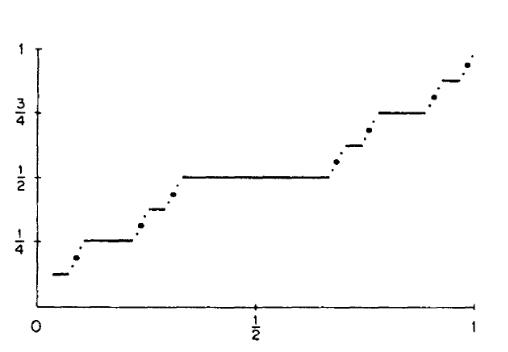
\includegraphics[scale = 0.5]{cantor_function.png}}
\end{minipage}
\caption{\footnotesize{\textbf{The Cantor Function \citep{reed1980methods}}}}
\label{fig: cantor_function}
\end{figure}




This example shows that the classical derivative $F'(x) := \lim_{h\rightarrow 0}\frac{F(x+h)−F (x)}{h}$ of a function has some defects; \emph{it
cannot ``see" some of the variation of a continuous monotone function} such as the Cantor function.
\end{remark}

\item \begin{remark}
In view of this counterexample, we see that we need to add \emph{an additional hypothesis} to \emph{\textbf{the continuous monotone} non-increasing function} $F$ before we can recover the second fundamental theorem. One such hypothesis is \emph{\textbf{absolute continuity}}.
\end{remark}


\item \begin{definition}
A function $F : \bR \rightarrow \bR$ is \emph{\textbf{continuous}} if, for every $\epsilon > 0$ and $x_0 \in \bR$, there exists a $\delta > 0$ such that $\abs{F(b) - F (a)} \le \epsilon$ whenever $(a, b)$ is an interval of length at most $\delta$ that contains $x_0$.
\end{definition}

\begin{definition}
A function $F : \bR \rightarrow \bR$ is \emph{\textbf{uniformly continuous}} if, for every $\epsilon > 0$, there exists a $\delta > 0$ such that $\abs{F(b) - F (a)} \le \epsilon$ whenever $(a, b)$  is an interval of length at most $\delta$.
\end{definition}

\item \begin{definition} (\textbf{\emph{Absolute Continuity}})\\
A function $F : \bR \rightarrow \bR$ is said to be \textbf{\emph{absolutely continuous}} if, for every $\epsilon > 0$, there exists a $\delta > 0$ such that $\sum_{j=1}^{n}\abs{F(b_j) - F(a_j)} \le \epsilon$ whenever $(a_1, b_1) \xdotx{,} (a_n, b_n)$ is a \textbf{finite collection of disjoint intervals} of \emph{\textbf{total length}} $\sum_{j=1}^{n}\abs{b_j - a_j}$ \emph{\textbf{at most $\delta$}}.
\end{definition}

\item \begin{proposition} The followings statements are true:
\begin{enumerate}
\item Every \textbf{absolutely continuous} function is \textbf{uniformly continuous} and therefore \textbf{continuous}.

\item Every \textbf{absolutely continuous} function is of \textbf{bounded variation} on every \textbf{compact} interval $[a, b]$. (Hint: first show this is true for any sufficiently small interval.) Thus, by the Local Bounded Variation Differentiation Theorem, absolutely continuous functions are \textbf{differentiable almost everywhere}.

\item Every \textbf{Lipschitz continuous} function is \textbf{absolutely continuous}.

\item The function $x \mapsto \sqrt{x}$ is absolutely continuous, but not Lipschitz continuous, on the interval $[0, 1]$.

\item \textbf{The Cantor function} is continuous, \textbf{monotone}, and \textbf{uniformly continuous}, but \textbf{not absolutely continuous}, on $[0, 1]$.

\item  If $f: \bR \rightarrow \bR$ is \textbf{absolutely integrable}, then the indefinite integral $F(x) := \int_{[-\infty,x]} f(y) dy$ is \textbf{absolutely continuous}, and $F$ is differentiable almost everywhere with $F'(x) = f(x)$ for almost every $x$.

\item The \textbf{sum} or \textbf{product} of two absolutely continuous functions on an interval $[a, b]$ remains absolutely continuous.
\end{enumerate}
\end{proposition}

\item \begin{remark}
We can draw the relative strength of different concepts on a \emph{compact interval} $[a, b]$.
\[
  \begin{tikzcd}
     \text{\emph{Lipschitz continuous}} \arrow{r}{}  \arrow{dr}{} & \text{\emph{absolutely continuous}} \arrow{d}{} \arrow{r}{} &  \text{\emph{uniformly continuous}}  \arrow{r}{}  &\text{\emph{continuous}} \\
     \text{\emph{convex}} \arrow{u}{} \arrow{ur}{}  \arrow{dr}{} & \text{\emph{locally bounded variation}} \arrow{dr}{} & & \\
\text{\emph{monotone}}  \arrow[rr, bend right]   \arrow{r}{\text{\emph{bounded}}}   & \text{\emph{bounded variation}}  \arrow{u}{} \arrow{r}{} & \text{\emph{differentiable a.e.}} &
  \end{tikzcd}
\] 
\begin{itemize}
\item \emph{\textbf{uniformly continuous}} $\not\rightarrow$ \emph{\textbf{absolutely continuous}}: See Cantor function example \citep{tao2011introduction}.
\item  \emph{\textbf{absolutely continuous}} $\not\rightarrow$ \emph{\textbf{Lipschitz continuous}}: $x \mapsto \sqrt{x}$
\end{itemize}
\end{remark}

\item \begin{proposition}
Absolutely continuous functions map \textbf{null sets} to \textbf{null sets}, i.e. if $F : \bR \rightarrow \bR$ is \textbf{absolutely continuous} and $E$ is a null set then $F(E) := \set{F(x): x \in E}$ is also a null set.
\end{proposition} 

\begin{exercise}
Show that the Cantor function does not have this property above.
\end{exercise}

\item For absolutely continuous functions, we can recover the second fundamental theorem of calculus:
\begin{theorem} (\textbf{Second Fundamental Theorem for Absolutely Continuous Functions}).\\
Let $F: [a, b] \rightarrow \bR$ be \underline{\textbf{absolutely continuous}}. Then
\begin{align*}
\int_{[a, b]}F'(x) dx = F(b) - F(a).
\end{align*} Note that $F'$ is \textbf{absolutely integrable}. 
\end{theorem}

\item \begin{proposition} (\textbf{Classification of Absolute Continuous Function})\\
A function $F: [a, b] \rightarrow \bR$ is \textbf{absolutely continuous} if and only if it takes the form 
\begin{align*}
F(x) = \int_{[a,x]} f(y) dy + C
\end{align*} for some \textbf{absolutely integrable} $f: [a, b] \rightarrow \bR$ and a constant $C$.
\end{proposition}

\item \begin{remark}
We see that the \emph{\textbf{absolute continuity}} was used primarily in \emph{two ways}: 
\begin{enumerate}
\item firstly, to ensure \emph{\textbf{the almost everywhere existence}} of $F'$
\item to control \emph{an exceptional \textbf{null set} $E$}.
\end{enumerate}
It turns out that one can achieve the latter control by making \emph{a different hypothesis}, namely that \emph{the function $F$ is everywhere differentiable} rather than merely \emph{almost everywhere differentiable}. More
precisely, we have
\end{remark}

\item \begin{theorem} (\textbf{Second Fundamental Theorem of Calculus, again}).\\
Let $[a, b]$ be a compact interval of positive length, let $F: [a, b] \rightarrow \bR$ be a \textbf{differentiable} function, such that \textbf{$F'$ is absolutely integrable}. Then the Lebesgue integral 
\begin{align*}
\int_{[a, b]}F'(x) dx = F(b) - F(a).
\end{align*}
\end{theorem}

\item \begin{exercise}
Let $F: [-1, 1] \rightarrow \bR$ be the function defined by setting 
\begin{align*}
F(x) := x^2 \sin\paren{\frac{1}{x^3}} 
\end{align*} when $x$ is non-zero, and $F(0) := 0$. Show that $F$ is everywhere differentiable, but the deriative $F'$ is not absolutely integrable, and so the second fundamental theorem of calculus does not apply in this case (at least if we interpret $\int_{[a,b]} F'(x) dx$ using the absolutely convergent Lebesgue integral). 
\end{exercise}

\end{itemize}
\newpage
\bibliographystyle{plainnat}
\bibliography{reference.bib}
\end{document}